\subsection{Configure GBTx in transmitter/transceiver and widebus/FEC mode}
GBTx boards can be configured to operate as a transmitter or a transceiver, with
a communication protocol of widebus or FEC, by hardware pins.
There are a total of 4 pins;
these related pins are shown in \autoref{fig:gbt-txrx}.

GBTx operations mode is completely determined by these 4 pins (corresponding to
4 bits). The 4-bit operation modes are listed in \nameref{appx:4bit}.

\begin{figure}[!ht]
\centering
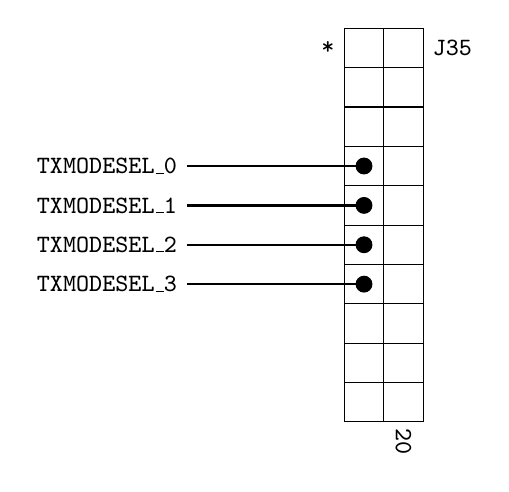
\begin{tikzpicture}
    % Pins
    \draw (0,0) rectangle (1,-5);
    \draw (0.5,0) to (0.5,-5);
    \draw (0,-0.5) to (1,-0.5);
    \draw (0,-1.5) to (1,-1.5);
    \draw (0,-2.5) to (1,-2.5);
    \draw (0,-3.5) to (1,-3.5);
    \draw (0,-4.5) to (1,-4.5);
    \draw (0,-1) to (1,-1);
    \draw (0,-2) to (1,-2);
    \draw (0,-3) to (1,-3);
    \draw (0,-4) to (1,-4);

    % PCB labels
    \coordinate (A) at (1,-0.25);
    \node at (A) [right] {\small\texttt{J35}};
    \coordinate (B) at (0,-0.25);
    \node at (B) [left] {\small\texttt{*}};
    \coordinate (C) at (0.75,-5.25);
    \node at (C) [rotate=-90] {\small\texttt{20}};

    % operation mode configuration pins
    \draw [black,fill] (0.25,-1.75) circle [radius=0.1];
    \draw [black,fill] (0.25,-2.25) circle [radius=0.1];
    \draw [black,fill] (0.25,-2.75) circle [radius=0.1];
    \draw [black,fill] (0.25,-3.25) circle [radius=0.1];

    \draw [thick] (-2,-1.75) to (0.25,-1.75);
    \node  at (-2,-1.75) [left] {\small\texttt{TXMODESEL\_0}};
    \draw [thick] (-2,-2.25) to (0.25,-2.25);
    \node  at (-2,-2.25) [left] {\small\texttt{TXMODESEL\_1}};
    \draw [thick] (-2,-2.75) to (0.25,-2.75);
    \node  at (-2,-2.75) [left] {\small\texttt{TXMODESEL\_2}};
    \draw [thick] (-2,-3.25) to (0.25,-3.25);
    \node  at (-2,-3.25) [left] {\small\texttt{TXMODESEL\_3}};
\end{tikzpicture}
\caption{
    Schematic showing all 4 related configuration pins.
    Note that the right column is a common ground.
    To switch a pin \emph{off}, connect it to a common ground pin.
}
\label{fig:gbt-txrx}
\end{figure}
